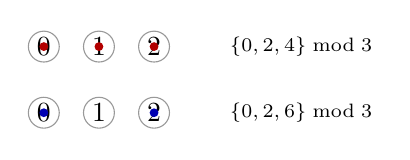
\begin{tikzpicture}[x=0.7cm,y=0.7cm]
\foreach \i in {0,1,2}{
  \draw[black!40] (\i,1.2) circle (0.28);
  \node at (\i,1.2) {$\i$};
}
\fill[red!70!black] (0,1.2) circle (0.08);
\fill[red!70!black] (2,1.2) circle (0.08);
\fill[red!70!black] (1,1.2) circle (0.08);
\node[font=\scriptsize,anchor=west] at (3.2,1.2) {$\{0,2,4\}\bmod 3$};
\foreach \i in {0,1,2}{
  \draw[black!40] (\i,0) circle (0.28);
  \node at (\i,0) {$\i$};
}
\fill[blue!70!black] (0,0) circle (0.08);
\fill[blue!70!black] (2,0) circle (0.08);
\node[font=\scriptsize,anchor=west] at (3.2,0) {$\{0,2,6\}\bmod 3$};
\end{tikzpicture}
